\section{伴随方程}
\label{sec:odesens-adjoint}

设参数有$p$个，而我们只关心由解算出的一个数，比如终点状态的某个函数。用式~\eqref{eq:odesens-parameter-variational}求梯度，就要解一个$n\times p$的矩阵方程，相当于$p$个线性系统。$p$很大时这难以承受，而我们要的只是一个数对$p$个参数的导数。能不能只解一次方程？

\paragraph{主要思想}
设目标函数同时含终端项和沿途的运行项：
\begin{equation}
 J(\bm{\theta})=\psi\bigl(\bm{x}(T),\bm{\theta}\bigr)+\int_{t_0}^{T}\ell\bigl(t,\bm{x}(t),\bm{\theta}\bigr)\,\mathrm{d}t,
 \label{eq:odesens-objective}
\end{equation}
其中$\bm{x}$解$\dot{\bm{x}}=\bm{f}(t,\bm{x},\bm{\theta})$，$\bm{x}(t_0)=\bm{x}_0(\bm{\theta})$。沿方向$\bm{w}$求导，$\bm{z}=\bm{P}\bm{w}$解变分方程，得到
\[
 \mathrm{D}J[\bm{w}]=\langle\nabla_{\bm{x}}\psi,\bm{z}(T)\rangle+\langle\nabla_{\bm{\theta}}\psi,\bm{w}\rangle+\int_{t_0}^{T}\bigl(\langle\nabla_{\bm{x}}\ell,\bm{z}\rangle+\langle\nabla_{\bm{\theta}}\ell,\bm{w}\rangle\bigr)\,\mathrm{d}t.
\]
麻烦的是$\bm{z}$，每换一个$\bm{w}$都要重解。

解决办法来自一个恒等式。设$\bm{z}$解$\dot{\bm{z}}=\bm{A}\bm{z}$，$\bm{\lambda}$解$\dot{\bm{\lambda}}=-\bm{A}^{\top}\bm{\lambda}$，则
\[
 \frac{\mathrm{d}}{\mathrm{d}t}\langle\bm{\lambda},\bm{z}\rangle=\langle-\bm{A}^{\top}\bm{\lambda},\bm{z}\rangle+\langle\bm{\lambda},\bm{A}\bm{z}\rangle=0.
\]
配对$\langle\bm{\lambda},\bm{z}\rangle$沿时间不变。如果$\bm{\lambda}$在终点等于目标的梯度，那么
\[
 \langle\nabla\psi,\bm{z}(T)\rangle=\langle\bm{\lambda}(t_0),\bm{z}(t_0)\rangle.
\]
于是问题转移到了起点：$\bm{z}(t_0)$是已知的。代价是$\bm{\lambda}$的条件给在终点，要从$T$反向解回$t_0$，图~\ref{fig:odesens-adjoint-scheme}是这个结构的示意。

\begin{BookInlineFigure}
  \centering
  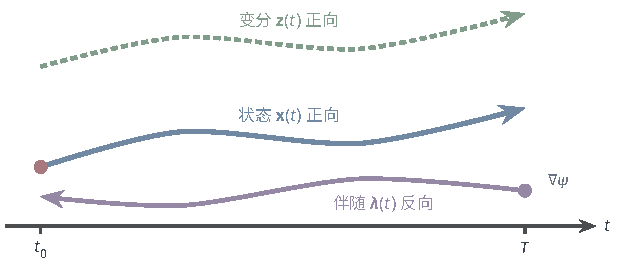
\includegraphics[width=105.2mm]{figures/06-differential-equations/01-ordinary-differential-equations/tikz/odesens-adjoint-scheme/figure.pdf}
  \caption{伴随计算的结构。状态$\bm{x}$从红色初值正向求解。变分$\bm{z}$（绿色虚线）也是正向的，每个方向都要解一次，伴随方法用不到它。伴随$\bm{\lambda}$（紫）从终点条件$\nabla\psi$出发反向求解，只解一次。配对$\langle\bm{\lambda},\bm{z}\rangle$在无运行项、无输入项时沿时间不变。}
  \label{fig:odesens-adjoint-scheme}
\end{BookInlineFigure}

一般情形多了非齐次项，只要在$\bm{\lambda}$的方程里补上运行项的梯度。在变分方程上演算，就得到下面的定理。

\begin{theorem}[伴随表示]
\label{thm:odesens-adjoint}
设$\bm{f}$满足定理~\ref{thm:odesens-differentiable}的条件，$\bm{x}_0(\bm{\theta})$、$\psi$连续可微，$\ell$对$t$可测、对$(\bm{x},\bm{\theta})$连续可微，且其导数在管道内被可积函数控制。设$\bm{A},\bm{B}$由式~\eqref{eq:odesens-coefficients}定义。令$\bm{\lambda}:[t_0,T]\to\mathbb{R}^{n}$是反向线性问题
\begin{equation}
 \dot{\bm{\lambda}}=-\bm{A}(t)^{\top}\bm{\lambda}-\nabla_{\bm{x}}\ell\bigl(t,\bm{x}(t),\bm{\theta}\bigr),\qquad
 \bm{\lambda}(T)=\nabla_{\bm{x}}\psi\bigl(\bm{x}(T),\bm{\theta}\bigr)
 \label{eq:odesens-adjoint}
\end{equation}
的解。则$J$在$\bm{\theta}$处可微，且
\begin{equation}
 \begin{aligned}
 \nabla J(\bm{\theta})={}&\nabla_{\bm{\theta}}\psi+\bigl[\partial_{\bm{\theta}}\bm{x}_0(\bm{\theta})\bigr]^{\top}\bm{\lambda}(t_0)\\
 &+\int_{t_0}^{T}\bigl[\bm{B}(t)^{\top}\bm{\lambda}(t)+\nabla_{\bm{\theta}}\ell\bigr]\,\mathrm{d}t.
 \end{aligned}
 \label{eq:odesens-adjoint-gradient}
\end{equation}
\end{theorem}

\begin{proof}
可微性由定理~\ref{thm:odesens-differentiable}、$\psi$的可微性以及该定理证明第四步那样的控制收敛论证得到，方向导数正是前面写出的$\mathrm{D}J[\bm{w}]$。式~\eqref{eq:odesens-adjoint}是系数可积的线性方程，在$[t_0,T]$上有唯一的绝对连续解。

设$\bm{z}$解方向$\bm{w}$的变分方程~\eqref{eq:odesens-variational}，起点取$(\partial_{\bm{\theta}}\bm{x}_0)\bm{w}$。计算配对的导数，$\bm{A}$的项相消，几乎处处有
\[
 \frac{\mathrm{d}}{\mathrm{d}t}\langle\bm{\lambda},\bm{z}\rangle=-\langle\nabla_{\bm{x}}\ell,\bm{z}\rangle+\langle\bm{\lambda},\bm{B}\bm{w}\rangle.
\]

从$t_0$到$T$积分，并代入$\bm{\lambda}(T)=\nabla_{\bm{x}}\psi$，移项得
\[
 \langle\nabla_{\bm{x}}\psi,\bm{z}(T)\rangle+\int_{t_0}^{T}\langle\nabla_{\bm{x}}\ell,\bm{z}\rangle\,\mathrm{d}t=\langle\bm{\lambda}(t_0),\bm{z}(t_0)\rangle+\int_{t_0}^{T}\langle\bm{\lambda},\bm{B}\bm{w}\rangle\,\mathrm{d}t.
\]
左边正是$\mathrm{D}J[\bm{w}]$中含$\bm{z}$的部分。代回$\mathrm{D}J[\bm{w}]$，右端对$\bm{w}$线性，读出系数就是式~\eqref{eq:odesens-adjoint-gradient}。
\end{proof}

称$\bm{\lambda}$为\term{伴随变量}（adjoint variable），式~\eqref{eq:odesens-adjoint}为\term{伴随方程}（adjoint equation）。式~\eqref{eq:odesens-adjoint-gradient}的各项对应目标导数的三个来源：含$\nabla_{\bm{\theta}}\psi$与$\nabla_{\bm{\theta}}\ell$的项是目标函数显含参数的部分；含$\bm{\lambda}(t_0)$的项是初值对参数的依赖；含$\bm{B}$的项是右端对参数的依赖。

\paragraph{$\bm{\lambda}$的含义}
无运行项时，比较式~\eqref{eq:odesens-adjoint}与式~\eqref{eq:odesens-initial-variational}，得到
\begin{equation}
 \bm{\lambda}(t)=\bm{\Phi}(T,t)^{\top}\nabla_{\bm{x}}\psi\bigl(\bm{x}(T)\bigr).
 \label{eq:odesens-adjoint-pullback}
\end{equation}
也就是说，$\bm{\lambda}(t)$是目标函数对时刻$t$状态的梯度：如果在时刻$t$把状态推动$\bm{v}$，目标函数的一阶变化是$\langle\bm{\lambda}(t),\bm{v}\rangle$。带运行项时含义相同，只是目标函数换成从$t$到$T$的累计。变分$\bm{z}$回答“推一下起点，后面怎么变”，伴随$\bm{\lambda}$回答“后面的目标，对前面每一刻有多敏感”，一个前传，一个后传。

\begin{example}[Logistic方程上的配对]
\label{ex:odesens-adjoint-logistic}
继续$\dot{x}=\theta x(1-x)$，$\theta=1$，$x_0=1/4$，$T=\ln3$，取$J=x(T)$，即$\psi(x)=x$，$\ell=0$。伴随方程是$\dot{\lambda}=-(1-2x)\lambda$，$\lambda(T)=1$。

记$f(x)=x(1-x)$。对$1/f(x(t))$求导，得到
\[
 \frac{\mathrm{d}}{\mathrm{d}t}\,\frac{1}{f(x)}=-\frac{1-2x}{f(x)}.
\]
所以$1/f(x(t))$满足伴随方程的齐次形式，配上终端条件，得
\[
 \lambda(t)=\frac{f(x(T))}{f(x(t))}.
\]
代入数据，$f(x(T))=1/4$，所以$\lambda(0)=\dfrac{1/4}{3/16}=\dfrac43$，这就是初值导数$S(T)$，与式~\eqref{eq:odesens-adjoint-pullback}一致。

对$\theta$的导数，$B(t)=f(x(t))$，所以
\[
 \lambda(t)B(t)=f(x(T))=\frac14\quad\text{（对所有}\ t\text{）}.
\]
积分得到$\partial_\theta J=\tfrac14\ln3\approx0.2747$，与例~\ref{ex:odesens-parameter-derivative}的$P(\ln3)$相同。
\end{example}

图~\ref{fig:odesens-adjoint-pairing}(a)中，$z=S(t)$从$1$升到$4/3$，$\lambda$从$4/3$降到$1$，乘积始终是$4/3$，这正是配对不变的数值表现。(b)显示伴随变量和被积函数的具体形状。

\begin{BookInlineFigure}
  \centering
  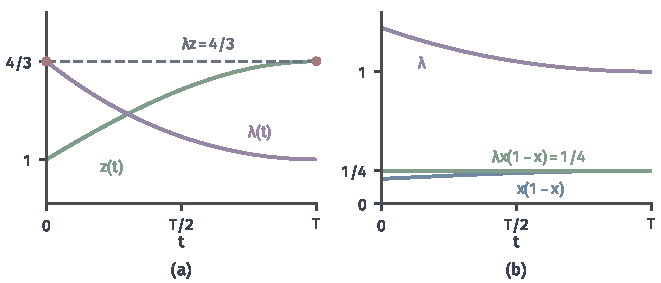
\includegraphics[width=112mm]{figures/06-differential-equations/01-ordinary-differential-equations/matplotlib/odesens-adjoint-pairing/figure.pdf}
  \caption{Logistic方程上的变分与伴随，$x_0=1/4$，$T=\ln3$，$J=x(T)$，数值积分得到。(a)前向的$z(t)=S(t)$（绿）与反向的$\lambda(t)$（紫），灰色虚线是乘积$\lambda z\equiv4/3$。红点是$\lambda(0)=z(T)=4/3$。(b)$\lambda$（紫）、$B=x(1-x)$（蓝）及其乘积（绿），乘积恒为$1/4$。}
  \label{fig:odesens-adjoint-pairing}
\end{BookInlineFigure}

\begin{example}[三个来源逐项核对]
\label{ex:odesens-adjoint-three}
取$\dot{x}=\theta x$，$x(0)=\theta$，$T=1$，
\[
 J(\theta)=\int_0^1\Bigl(x(t)+\frac12\theta^2\Bigr)\mathrm{d}t.
\]
解是$x=\theta\mathrm{e}^{\theta t}$，直接积分得$J=\mathrm{e}^{\theta}-1+\tfrac12\theta^2$，所以$J'(1)=\mathrm{e}+1$。

用伴随计算，取$\theta=1$。这里$\psi=0$，$\ell=x+\tfrac12\theta^2$，$A=1$，$B=x=\mathrm{e}^{t}$。伴随方程$\dot{\lambda}=-\lambda-1$、$\lambda(1)=0$的解是
\[
 \lambda(t)=\mathrm{e}^{1-t}-1.
\]

三项贡献依次是：
\[
 \begin{aligned}
 \text{初值：}&\ \partial_\theta x_0\,\lambda(0)=1\cdot(\mathrm{e}-1)=\mathrm{e}-1,\\
 \text{右端：}&\ \int_0^1\lambda B\,\mathrm{d}t=\int_0^1\bigl(\mathrm{e}-\mathrm{e}^{t}\bigr)\mathrm{d}t=1,\\
 \text{目标：}&\ \int_0^1\partial_\theta\ell\,\mathrm{d}t=\int_0^1\theta\,\mathrm{d}t=1.
 \end{aligned}
\]
相加得$\mathrm{e}+1$，与直接求导的结果相同。
\end{example}

\paragraph{计算过程}
下面把伴随方法写成计算过程，并同时在第~\ref{sec:odesens-parameter-derivative}节的分段输入例子上执行：$\dot{x}=-x+g(t)$，$x_0=0$，$T=2$，$g$在$[0,1)$、$[1,2)$上分别取$\theta_1=1$、$\theta_2=2$，目标是$J=\tfrac12x(2)^2$。

\needspace{6\baselineskip}
\paragraph{变量}
需要的量是：
\begin{itemize}
 \item 状态轨迹$\bm{x}(t)\in\mathbb{R}^{n}$，要保存下来或能够重新算出，供反向求解时使用；
 \item 伴随变量$\bm{\lambda}(t)\in\mathbb{R}^{n}$；
 \item 累积梯度$\bm{G}(t)\in\mathbb{R}^{p}$，表示$[t,T]$这段时间已经计入的梯度贡献。
\end{itemize}

\paragraph{初始化}
参数$\bm{\theta}$、初值$\bm{x}_0(\bm{\theta})$给定。例中$\bm{\theta}=(1,2)$，$x_0=0$，$\partial_{\bm{\theta}}x_0=\bm{0}$。

\needspace{6\baselineskip}
\paragraph{计算步骤}
\begin{enumerate}
 \item \emph{正向求解状态}，得到$\bm{x}(t)$，$t\in[t_0,T]$。例中逐段积分，
 \[
  x(1)=1-\mathrm{e}^{-1}=0.63212,\qquad x(2)=2+\bigl(x(1)-2\bigr)\mathrm{e}^{-1}=1.49679.
 \]

 \item \emph{设置终端条件}。令
 \[
  \bm{\lambda}(T)=\nabla_{\bm{x}}\psi(\bm{x}(T),\bm{\theta}),\qquad\bm{G}(T)=\bm{0}.
 \]
 例中$\lambda(2)=x(2)=1.49679$。

 \item \emph{反向求解伴随}。由式~\eqref{eq:odesens-adjoint}从$T$积到$t_0$，同时累积
 \[
  \dot{\bm{G}}=-\bigl[\bm{B}(t)^{\top}\bm{\lambda}(t)+\nabla_{\bm{\theta}}\ell\bigr].
 \]
 例中$A=-1$，无运行项，方程为$\dot{\lambda}=\lambda$，所以$\lambda(t)=x(2)\mathrm{e}^{t-2}$，
 \[
  \lambda(1)=0.55064,\qquad\lambda(0)=0.20257.
 \]

 \item \emph{合成梯度}。由式~\eqref{eq:odesens-adjoint-gradient}，
 \[
  \nabla J=\bm{G}(t_0)+\nabla_{\bm{\theta}}\psi+\bigl[\partial_{\bm{\theta}}\bm{x}_0\bigr]^{\top}\bm{\lambda}(t_0).
 \]
 例中$B$在$[0,1)$上为$(1,0)$，在$[1,2)$上为$(0,1)$，初值项为零，
 \[
  \partial_{\theta_1}J=\int_0^1\lambda\,\mathrm{d}t=0.34807,\qquad
  \partial_{\theta_2}J=\int_1^2\lambda\,\mathrm{d}t=0.94615.
 \]
\end{enumerate}

积分到$t_0$，计算结束。最终得到$\nabla J(1,2)=(0.34807,\,0.94615)$。用第~\ref{sec:odesens-parameter-derivative}节的$P_j(2)$核对，$\partial_{\theta_j}J=x(2)P_j(2)$，分别是$1.49679\times0.23254$与$1.49679\times0.63212$，结果相同。

图~\ref{fig:odesens-adjoint-gradient}把输入分成$20$段。一次反向积分给出全部$20$个偏导数，红点是逐分量差分的结果，最大差约$2\times10^{-7}$。越晚的输入对$J$的影响越大，因为$\lambda(t)$在靠近$T$时最大。

\begin{BookInlineFigure}
  \centering
  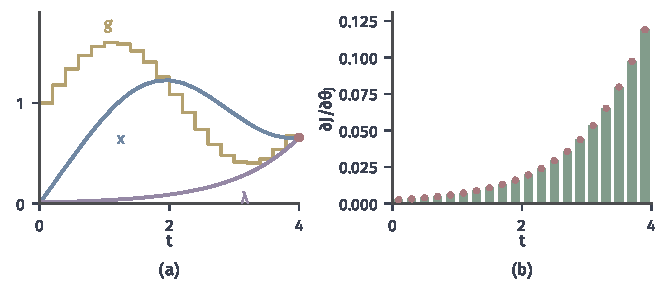
\includegraphics[width=112mm]{figures/06-differential-equations/01-ordinary-differential-equations/matplotlib/odesens-adjoint-gradient/figure.pdf}
  \caption{一次反向求解给出全部偏导数。方程$\dot{x}=-x+g$，$x_0=0$，$g$在$[0,4]$上分$20$段取常值（黄），$J=\tfrac12x(4)^2$。(a)状态$x$（蓝）与伴随$\lambda(t)=x(4)\mathrm{e}^{t-4}$（紫），红点是终端值。(b)绿色柱是伴随计算的$20$个偏导数，红点是逐分量中心差分。}
  \label{fig:odesens-adjoint-gradient}
\end{BookInlineFigure}

\paragraph{代价与失效情形}
表~\ref{tab:odesens-forward-adjoint}比较了前向与反向两种求导方式，其中$p$是参数个数，$k$是目标函数的个数。

\begin{BookInlineTable}
  \centering
  \caption{前向变分与反向伴随的代价对比。线性系统指沿同一条轨迹的$n$维线性初值问题。}
  \label{tab:odesens-forward-adjoint}
  \begin{tabular}{p{22mm}p{38mm}p{38mm}}
    \toprule
    & 前向变分 & 反向伴随 \\
    \midrule
    线性系统个数 & $p$个 & $k$个 \\
    是否保存轨迹 & 不需要，与状态同步 & 需要保存或重算 \\
    适合的情形 & 参数少、目标多 & 参数多、目标少 \\
    额外产出 & 完整的$\bm{P}(t)$ & 每一时刻的$\bm{\lambda}(t)$ \\
    \bottomrule
  \end{tabular}
\end{BookInlineTable}

伴随的主要代价是轨迹的存储。反向积分时要用到$\bm{A}(t)$，也就要用到$\bm{x}(t)$，长时间问题要在内存和重算之间权衡。$\bm{\lambda}$的大小也受放大因子控制：由式~\eqref{eq:odesens-adjoint-pullback}，
\[
 \lVert\bm{\lambda}(t)\rVert_2\leq\lVert\bm{\Phi}(T,t)\rVert_2\lVert\nabla\psi\rVert_2.
\]
敏感的问题里梯度本身就很大。

数值计算时还要注意，定理给的是连续问题的梯度。把伴随方程离散后算出的结果，一般不等于对离散格式求导的结果，两者只在步长趋于零时一致。定理的光滑性条件也不能省：右端在解经过的地方有$\lvert x\rvert$那样的折点时，$J$可能不可微。

得到梯度只是第一步，用它更新参数属于优化算法，可参考\BookChapterRef{chap:first-order-methods}{卷五第6章“一阶方法”}。当未知量是控制函数而不是有限维参数时，最优性条件需要更多工具，可参考\BookChapterRef{chap:continuous-time-optimal-control}{卷十第6章“连续时间最优控制”}。
